\chapter{IMPLEMENTATION AND TESTING}

\section{System Implementation}
The cyber-physical snooker ball identification and laser positioning platform is implemented as six modular subsystems spanning mechanical rig fabrication, embedded power electronics, deep learning computer vision, RESTful middleware, 3D WebGL visualization, and autonomous refereeing.

\subsection{Module 1: Physical Table and Overhead PVC Gantry Construction}
To create a dependable, rigid experimental platform that conforms to institutional laboratory space constraints while faithfully replicating professional snooker dynamics, a custom snooker table and overhead gantry were constructed.

\subsection{Table Specifications and Playing Surface}
The physical snooker table features an active playing surface measuring:
\begin{itemize}
    \item \textbf{Internal Playing Width ($W_{\text{table}}$):} $1168.4\,\text{mm}$ ($46.0\,\text{inches}$)
    \item \textbf{Internal Playing Length ($L_{\text{table}}$):} $2341.88\,\text{mm}$ ($92.2\,\text{inches}$)
    \item \textbf{Aspect Ratio:} Exactly $1:2.004$, mirroring regulation cue sports proportions.
    \item \textbf{Cushion Railing and Pockets:} Six regulation pockets (four corner pockets and two center pockets) lined with drop nets and leather impact bevels.
    \item \textbf{Cloth and Baize:} High-density tournament green wool-nylon blend felt stretched over a leveled bed, providing uniform rolling resistance.
\end{itemize}

\subsection{Structural PVC Overhead Gantry}
To eliminate floor obstructions around the playing perimeter while ensuring complete visual coverage of the $1168.4 \times 2341.88\,\text{mm}$ surface, an overhead structural gantry was engineered using high-grade $1.0\text{-inch}$ Schedule-40 Polyvinyl Chloride (PVC) piping. 

As shown in Figures \ref{fig:rig_setup} and \ref{fig:rig_overhead}, the gantry structure features:
\begin{itemize}
    \item \textbf{Vertical Clear Height:} $1315.15\,\text{mm}$ ($51.78\,\text{inches}$) clearance from the table bed to the overhead transverse crossbars.
    \item \textbf{Four Corner Uprights:} Dual-tube vertical columns reinforced with transverse T-connectors to prevent mechanical sway, torsion, and vibration.
    \item \textbf{Overhead Transverse Beam:} Houses the central downward-facing Full HD camera mount, aligned with the geometric center of the table.
\end{itemize}

\begin{figure}[H]
    \centering
    \begin{subfigure}[b]{0.48\textwidth}
        \centering
        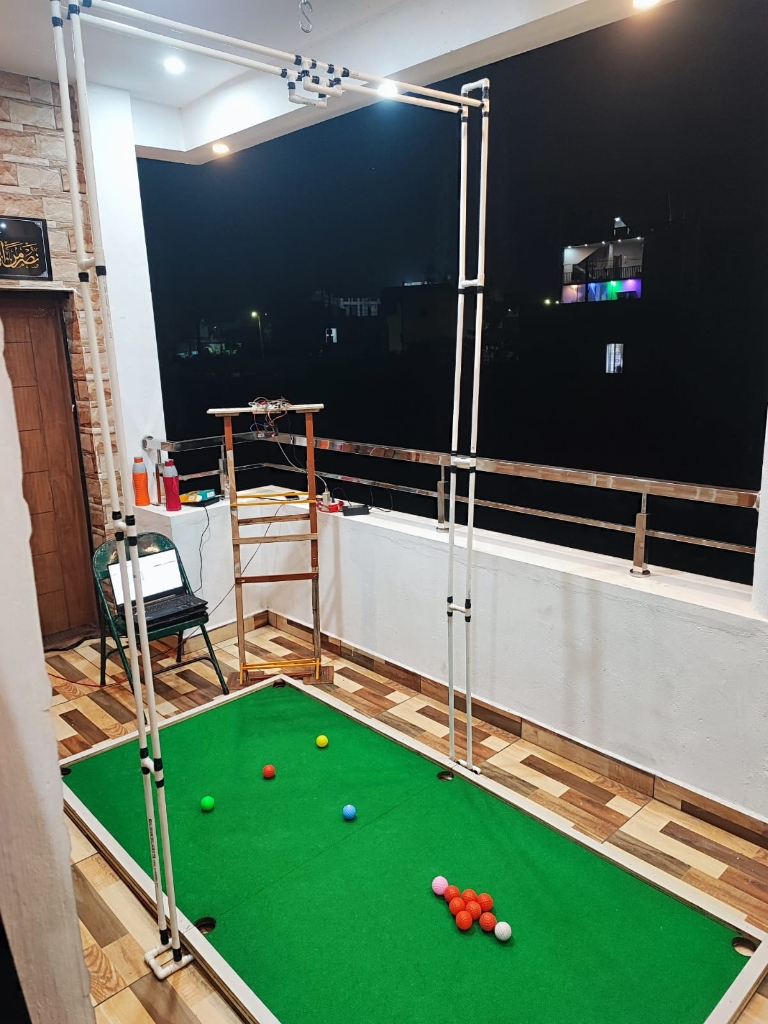
\includegraphics[width=\textwidth]{rig_setup_perspective.jpg}
        \caption{Perspective view of PVC gantry, lighting, and table}
        \label{fig:rig_setup}
    \end{subfigure}
    \hfill
    \begin{subfigure}[b]{0.48\textwidth}
        \centering
        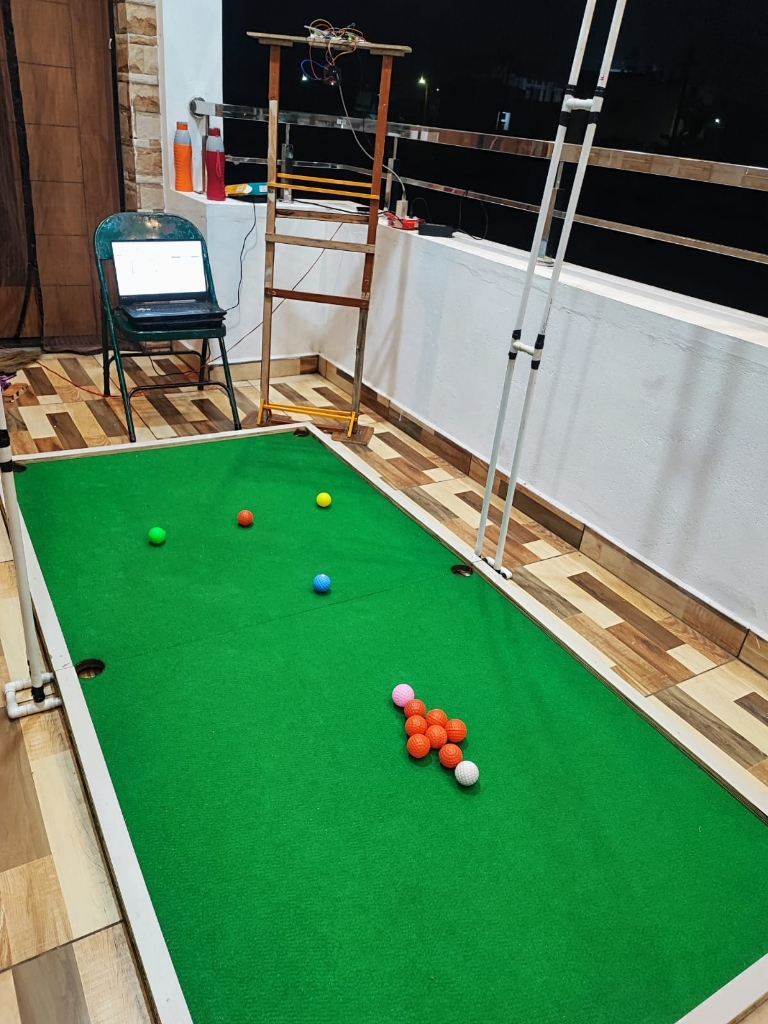
\includegraphics[width=\textwidth]{rig_gantry_overhead.jpg}
        \caption{Overhead view showing top-down camera frame}
        \label{fig:rig_overhead}
    \end{subfigure}
    \caption{Physical Hardware Rig: Custom Table, Overhead PVC Gantry, and Illumination}
    \label{fig:physical_hardware_rig}
\end{figure}

\subsection{Active Ball Set and Color Strategy}
In our prototype setup, a specialized ball configuration was adopted:
\begin{itemize}
    \item \textbf{Diameter:} Regulation $52.5\,\text{mm}$ phenolic resin spheres.
    \item \textbf{Object Balls (Orange Set):} High-visibility dimpled/smooth orange balls were deployed in place of traditional dark red balls. As illustrated in Figures \ref{fig:table_topdown} and \ref{fig:table_overview}, orange spheres provide superior chrominance contrast against green tournament cloth, maximizing the signal-to-noise ratio in the YOLOv8 convolutional feature space.
    \item \textbf{Color Balls:} Standard tournament colors: White (Cue Ball), Yellow (2 pts), Green (3 pts), Blue (5 pts), and Pink (6 pts).
\end{itemize}

\begin{figure}[H]
    \centering
    \begin{subfigure}[b]{0.48\textwidth}
        \centering
        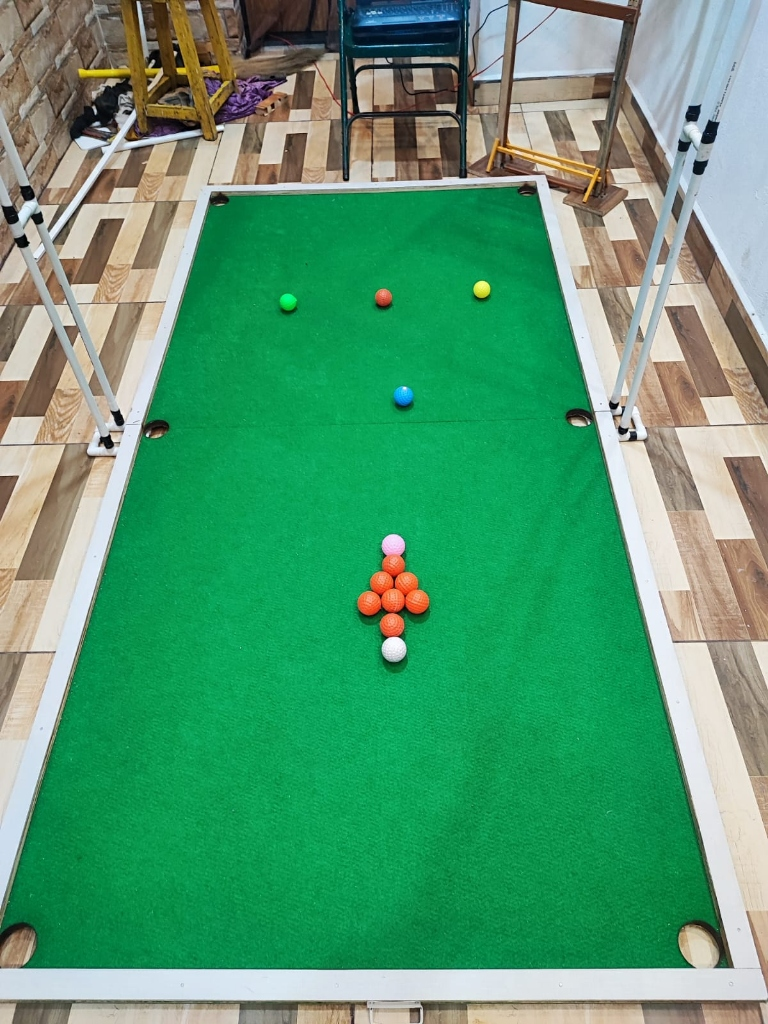
\includegraphics[width=\textwidth]{table_topdown_balls.jpg}
        \caption{Top-down longitudinal view of table cloth and rack}
        \label{fig:table_topdown}
    \end{subfigure}
    \hfill
    \begin{subfigure}[b]{0.48\textwidth}
        \centering
        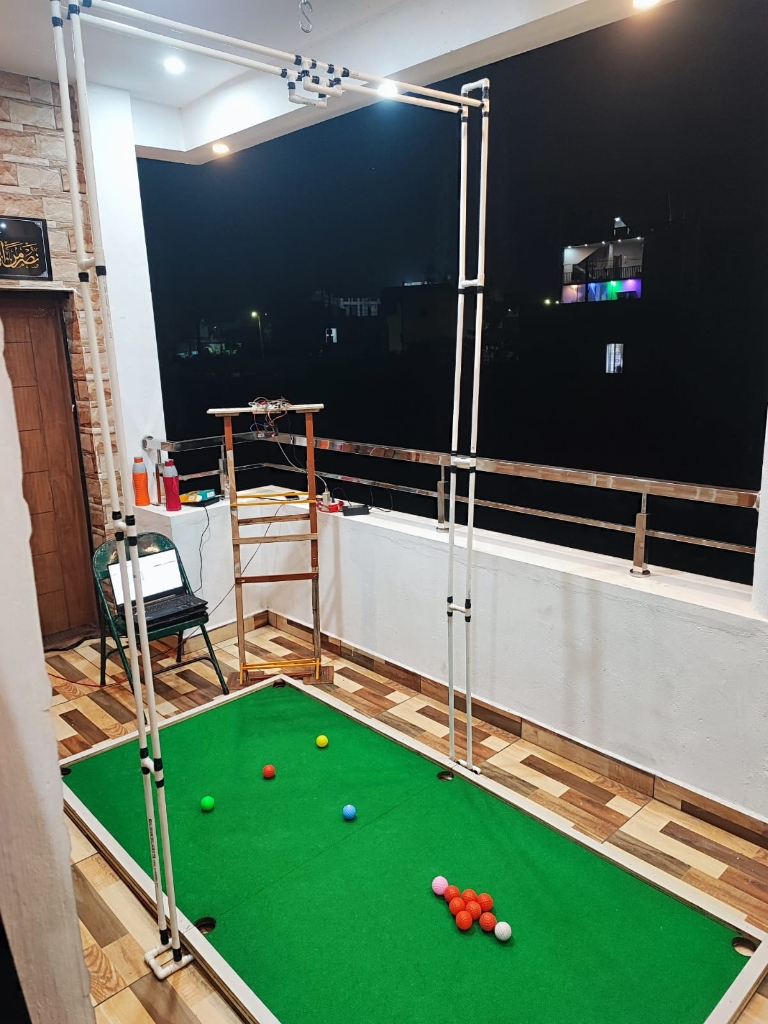
\includegraphics[width=\textwidth]{physical_table_overview.jpg}
        \caption{Overview of table, control laptop, and side rig}
        \label{fig:table_overview}
    \end{subfigure}
    \caption{Physical Snooker Playing Surface and Active Ball Set Deployment}
    \label{fig:physical_balls_table}
\end{figure}

\section{Embedded Hardware and Mechatronics Implementation}
The physical actuation and optical projection subsystem combines robust mechatronics, dedicated power regulation, high-current switching, and real-time microcontroller firmware. Figure \ref{fig:hardware_mechatronics_photos} shows the real physical assembly of both the dual-servo pan-tilt gimbal and the completed breadboard circuit.

\begin{figure}[H]
    \centering
    \begin{subfigure}[b]{0.48\textwidth}
        \centering
        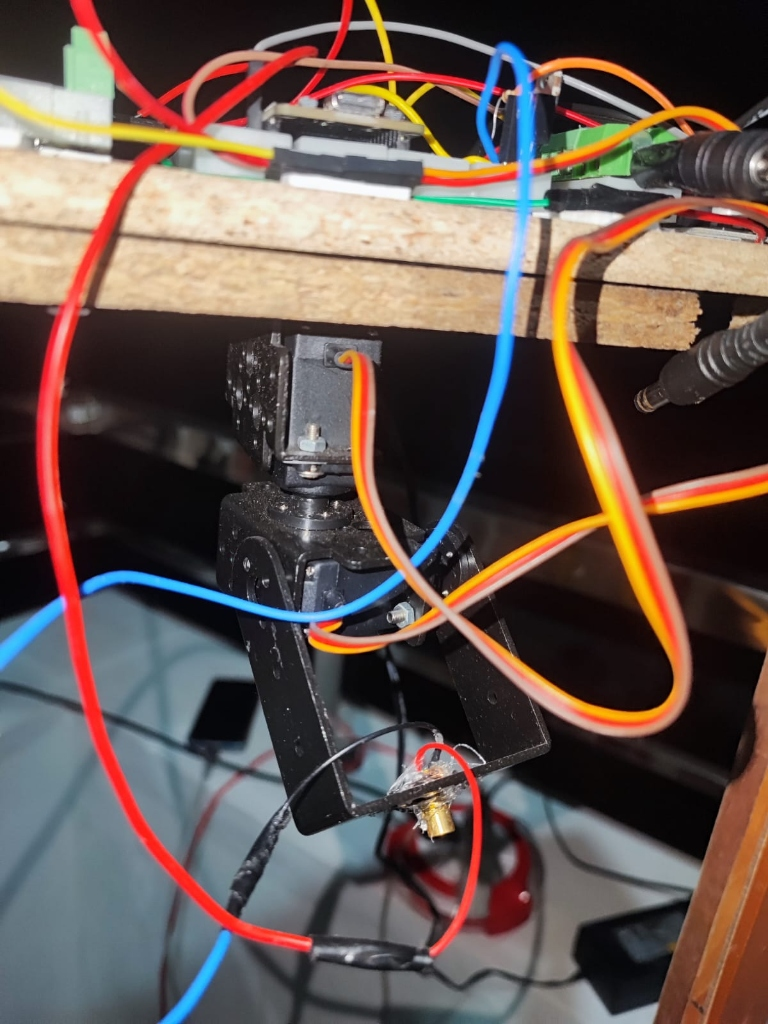
\includegraphics[width=\textwidth]{hardware_pantilt_assembly.jpg}
        \caption{Dual MG996R metal-gear servos in aluminum pan-tilt bracket with laser diode}
        \label{fig:hw_pantilt}
    \end{subfigure}
    \hfill
    \begin{subfigure}[b]{0.48\textwidth}
        \centering
        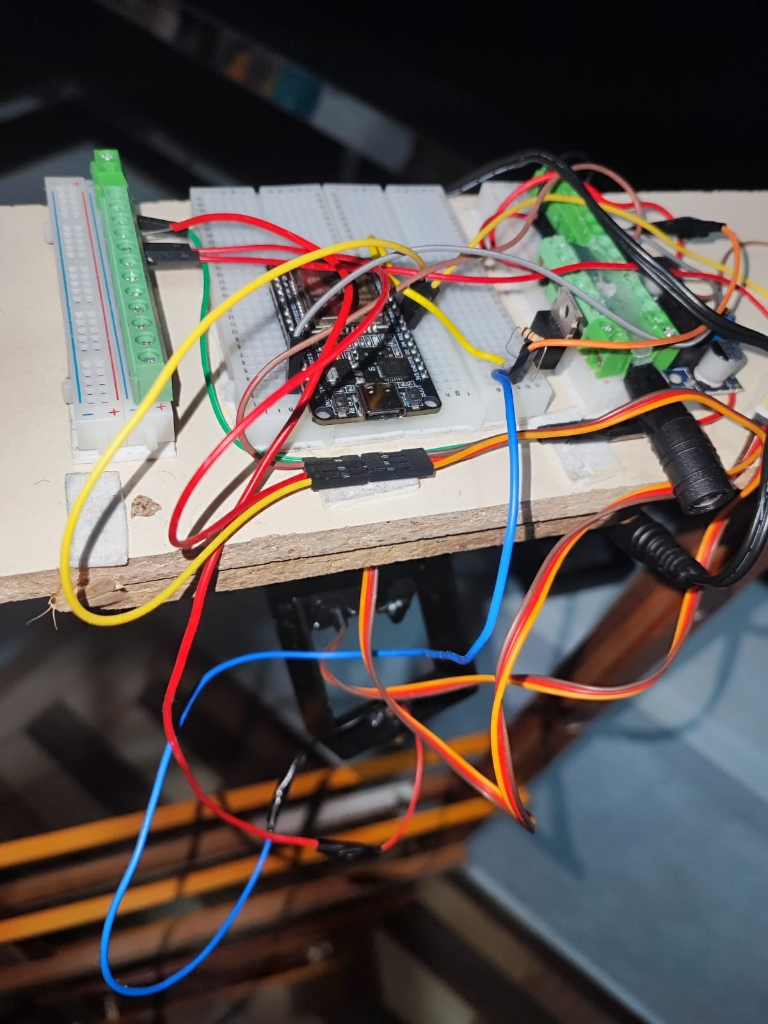
\includegraphics[width=\textwidth]{hardware_circuit_breadboard.jpg}
        \caption{Breadboard electronics: ESP32 Dev Kit, DC-DC buck converter, IRFZ44N MOSFET, and terminal blocks}
        \label{fig:hw_circuit}
    \end{subfigure}
    \caption{Physical Mechatronics and Embedded Circuit Assembly}
    \label{fig:hardware_mechatronics_photos}
\end{figure}

\subsection{Pan-Tilt Gimbal and MG996R Metal Gear Servos}
As shown in Figure \ref{fig:hw_pantilt}, the optical pointer is constructed using heavy-duty black anodized aluminum pan-tilt brackets suspended beneath the wooden side platform:
\begin{itemize}
    \item \textbf{High-Torque Metal Gear Servos:} Two TowerPro MG996R metal-gear servos provide the azimuth (Pan) and elevation (Tilt) motions. Compared to standard plastic-gear micro-servos, the MG996R features full steel and brass gearing delivering an exceptional stall torque of $11.0\,\text{kg}\cdot\text{cm}$ at $6.0\,\text{V}$. This completely eliminates the gear stripping, backlash play, and cantilevered sagging observed in lightweight servos over long table distances.
    \item \textbf{Laser Diode Mount:} A $650\,\text{nm}$ red focused dot laser diode module ($5\,\text{mW}$) is securely seated in the central bracket holder, locked with thermal adhesive to maintain bore-sight alignment across repeated rapid servo rotations.
\end{itemize}

\subsection{Circuit Architecture, Power Regulation, and MOSFET Switching}
The electronic control system shown in Figure \ref{fig:hw_circuit} is built across two solderless prototyping breadboards equipped with industrial screw terminal blocks for high-current routing:
\begin{enumerate}
    \item \textbf{12V 5A Master Power Supply:} A 12V 5A (60 Watts) switch-mode DC power adapter provides primary power via a standard $2.1\,\text{mm} \times 5.5\,\text{mm}$ barrel jack into the primary screw terminal block.
    \item \textbf{DC-DC Buck Converter (6.0V Bus):} Because the two MG996R servos draw up to $1.2\,\text{A}$ stall current each during acceleration, an onboard high-efficiency DC-to-DC step-down buck converter (LM2596 / XL4015) steps down the $12\,\text{V}$ input to a steady, regulated $6.0\,\text{V}$ DC bus. This isolated high-current bus directly feeds the servos, completely eliminating the voltage drops and brownout resets that occur when servos share a linear 5V logic regulator.
    \item \textbf{ESP32 Dev Kit Microcontroller:} The 30-pin ESP-WROOM-32 development board is powered through its VIN/USB port, sharing a common ground plane with the $6.0\,\text{V}$ and $12\,\text{V}$ supplies.
    \item \textbf{IRFZ44N Power MOSFET Laser Driver:} To isolate the ESP32 GPIO logic and ensure clean, high-speed switching of the laser diode without loading the microcontroller, an IRFZ44N N-Channel Power MOSFET ($V_{DSS} = 55\,\text{V}$, $I_D = 49\,\text{A}$, $R_{DS(on)} = 17.5\,\text{m}\Omega$) is deployed in a low-side switching configuration:
    \begin{itemize}
        \item The MOSFET Gate is driven by ESP32 GPIO 23.
        \item A $10\,\text{k}\Omega$ metal film pull-down resistor is wired between Gate and GND, ensuring that the gate is held securely at logic LOW ($0\,\text{V}$) during ESP32 bootup, flash programming, or Wi-Fi initialization.
        \item The Drain pin sinks the laser diode cathode, while the laser anode connects to the positive power rail through a current-limiting resistor.
        \item When GPIO 23 outputs HIGH ($3.3\,\text{V}$), the MOSFET channel fully conducts with negligible internal resistance, instantaneously illuminating the laser beam with maximum optical coherence.
    \end{itemize}
\end{enumerate}

\subsection{Embedded Firmware Architecture (ESP32 Station Mode)}
The embedded firmware executes on the ESP32 utilizing FreeRTOS tasks and the `ESP32Servo` library:
\begin{itemize}
    \item \textbf{Wi-Fi Station Mode:} The ESP32 connects directly to the dedicated local wireless network with static IP `10.21.46.190`, providing low-latency packet transmission ($\sim 34\,\text{ms}$).
    \item \textbf{Hardware Timer PWM:} Channels 0 and 1 on Timer 0 generate stable $50\,\text{Hz}$ PWM control pulses ($500\,\mu\text{s}$ to $2500\,\mu\text{s}$) on GPIO 18 (Pan) and GPIO 19 (Tilt) with 16-bit resolution.
    \item \textbf{RESTful Web Server:} Implements an asynchronous HTTP server handling \texttt{POST /move}, \texttt{GET /status}, and \texttt{GET /laser?state=0|1}.
    \item \textbf{Safety Watchdog:} Automatically shuts down the laser diode if no commands are received within $120\,\text{seconds}$, complying with optical eye-safety standards.
\end{itemize}

\section{Computer Vision Pipeline (YOLOv8s)}
Object detection is driven by Ultralytics YOLOv8s (Small), an anchor-free single-stage detector characterized by high detection precision and edge-device inference speed \cite{ref11, ref12}.

\subsection{Model Training and Dataset Annotation}
The model was fine-tuned on a custom dataset of 1,850 annotated snooker table images captured under varied lighting, ball positions, and cluster densities. Bounding boxes were manually annotated across six classes:
\begin{enumerate}
    \item \texttt{orange ball} (Object balls, 1 point)
    \item \texttt{white ball} (Cue ball)
    \item \texttt{yellow ball} (2 points)
    \item \texttt{green ball} (3 points)
    \item \texttt{blue ball} (5 points)
    \item \texttt{pink ball} (6 points)
\end{enumerate}
Training was executed on an NVIDIA GPU workstation over 100 epochs using the AdamW optimizer, cosine learning rate scheduling ($lr_0 = 0.01$), mosaic augmentation, and multi-scale resizing ($1024 \times 1024$ pixels).

\subsection{Inference and Non-Maximum Suppression (NMS)}
During live operation, raw camera frames are resized to $1024 \times 1024$ and fed to the YOLOv8s inference engine. Detections undergo Non-Maximum Suppression (NMS) with an IoU threshold of $0.45$ and a confidence threshold of $0.50$, outputting bounding boxes $(x_1, y_1, x_2, y_2)$, class label $c_k$, and prediction score $s_k$. Centroid pixel coordinates are computed as:
\begin{equation}
    u_c = \frac{x_1 + x_2}{2}, \quad v_c = \frac{y_1 + y_2}{2}
\end{equation}

\section{Backend Server Architecture (Flask)}
The backend system (\texttt{snooker\_web\_app.py}) is implemented using Python and Flask, orchestrating video stream processing, coordinate transformations, and REST communication with the ESP32.

\subsection{Video Streaming and Offline Fault Resilience}
The overhead camera feed is accessed via an RTSP/MJPEG network stream. To prevent server blocking during network drops or when the camera phone is switched off, a multi-threaded streaming proxy was implemented:
\begin{itemize}
    \item \textbf{Low Socket Timeout:} HTTP socket reads are capped at $1.2\,\text{seconds}$.
    \item \textbf{Offline Frame Cache:} If the live camera stream disconnects, the backend seamlessly serves a cached reference table image (`photo58.jpg`) annotated with an ``OFFLINE / CACHED FEED'' badge. This allows all web application tabs, 3D simulations, and calibration routines to remain fully operable without runtime crashes.
\end{itemize}

\subsection{API Routing}
Key REST endpoints exposed by the Flask backend include:
\begin{itemize}
    \item \texttt{GET /api/camera/stream}: Streams live MJPEG video frames to the web UI.
    \item \texttt{POST /api/table/corners}: Saves the four calibrated pixel corner fiducials and computes the $3 \times 3$ homography matrix $\mathbf{H}$.
    \item \texttt{POST /api/laser/move}: Computes spline-interpolated servo angles and dispatches an HTTP request to `http://10.21.46.190/move`.
    \item \texttt{POST /api/laser/nudge}: Applies micro-trim increments ($\pm 0.2^\circ$ or $\pm 1.0^\circ$) to current pan/tilt angles.
    \item \texttt{POST /api/referee/analyze\_shot}: Triggers YOLOv8 detection, compares pre/post states, and returns displaced ball vectors.
\end{itemize}

\section{Interactive 3D Digital Twin and User Interface}
The front-end user interface is implemented as a single-page responsive dashboard providing full supervisory control over the physical and virtual table states.

\subsection{Three.js 3D Virtual Table Twin}
Using Three.js WebGL, a geometrically accurate 3D model of the snooker table was developed:
\begin{itemize}
    \item Real-world metric dimensions ($1168.4 \times 2341.88\,\text{mm}$) scaled into 3D units.
    \item Six modeled regulation drop pockets with dark inner recesses.
    \item Tournament baulk line ($737\,\text{mm}$ from bottom cushion) and semi-circular 'D' zone ($292\,\text{mm}$ radius).
    \item Dynamically rendered 3D ball meshes positioned in real-time according to YOLO detections, colored accurately by class.
    \item Virtual laser ray projected from the top-right gantry mast to the selected target coordinate on the cloth, displaying live calculated pan/tilt angles.
    \item OrbitControls allowing free perspective orbiting, top-down bird's eye view, and player eye-level inspection.
\end{itemize}

\subsection{Tabbed Interface Modules}
As evidenced in Figures \ref{fig:ui_3d} to \ref{fig:ui_yolo}, the web application organizes system functionality into six intuitive tabs:
\begin{enumerate}
    \item \textbf{Tab 1 (3D Table View \& Click-to-Aim):} Displays the interactive 3D digital twin alongside a target positioning panel with quick preset buttons for pockets, center spots, and live fine-tuning nudge controls (Figures \ref{fig:ui_3d} and \ref{fig:ui_laser}).
    \item \textbf{Tab 2 (Camera \& Homography):} Features an interactive canvas where the referee clicks table corner pockets to compute and verify the homography matrix $\mathbf{H}$ (Figure \ref{fig:ui_homography}).
    \item \textbf{Tab 3 (Servo \& Laser Controls):} Exposes direct hardware sliders, IP configuration (`10.21.46.190`), ping latency diagnostics, and laser safety overrides (Figure \ref{fig:ui_servo}).
    \item \textbf{Tab 4 (Ball Detection \& YOLO):} Displays raw camera frames with overlaid YOLOv8 bounding boxes, detection confidence tags, metric $(X_w, Y_w)$ coordinates, and individual ``Aim Laser'' buttons for every ball (Figure \ref{fig:ui_yolo}).
    \item \textbf{Tab 5 (Foul Detection \& Autonomous Referee):} Displays real-time video motion percentages, automated pre/post shot state transitions, and a table of displaced balls with one-click laser restoration actions (Figure \ref{fig:ui_referee}).
    \item \textbf{Tab 6 (9-Point Calibration Wizard):} Guided interface for recording empirical servo angles across the nine reference table nodes to update the 2D bivariate cubic spline model (Figure \ref{fig:ui_calib}).
\end{enumerate}

\begin{figure}[H]
    \centering
    \begin{subfigure}[b]{0.48\textwidth}
        \centering
        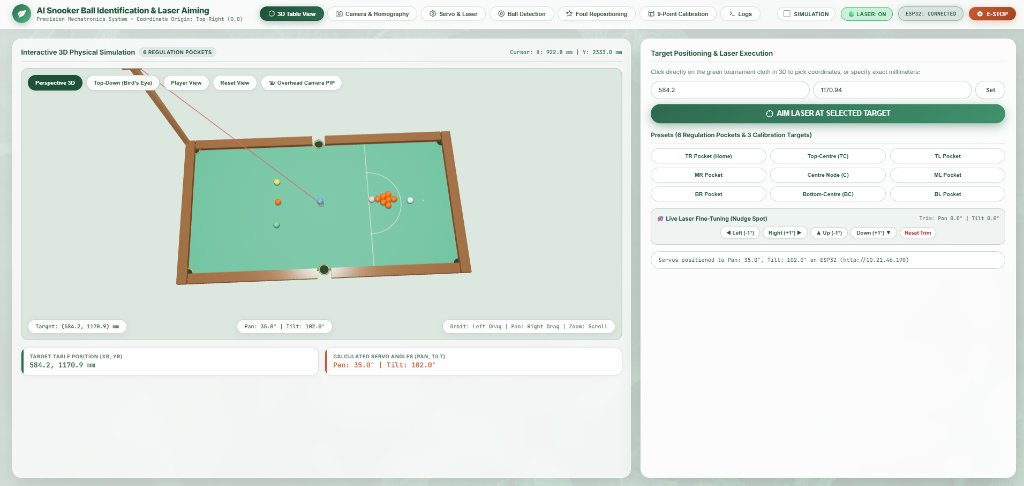
\includegraphics[width=\textwidth]{ui_3d_table.png}
        \caption{Tab 1: Interactive Three.js 3D Virtual Table Twin}
        \label{fig:ui_3d}
    \end{subfigure}
    \hfill
    \begin{subfigure}[b]{0.48\textwidth}
        \centering
        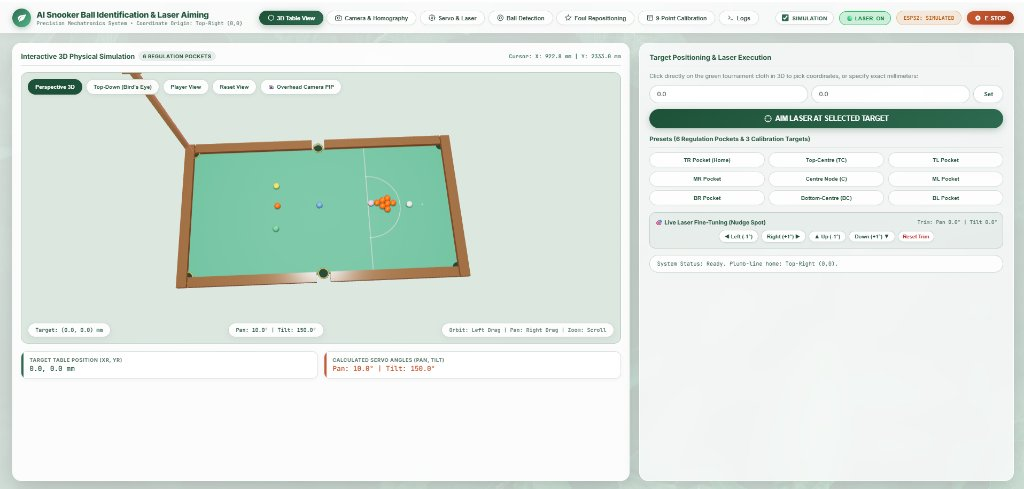
\includegraphics[width=\textwidth]{ui_laser_aiming.png}
        \caption{Tab 1: Target Positioning and Live Laser Aiming}
        \label{fig:ui_laser}
    \end{subfigure}
    \caption{Web Application Interface: 3D Simulation and Target Execution}
    \label{fig:ui_views_1}
\end{figure}

\begin{figure}[H]
    \centering
    \begin{subfigure}[b]{0.48\textwidth}
        \centering
        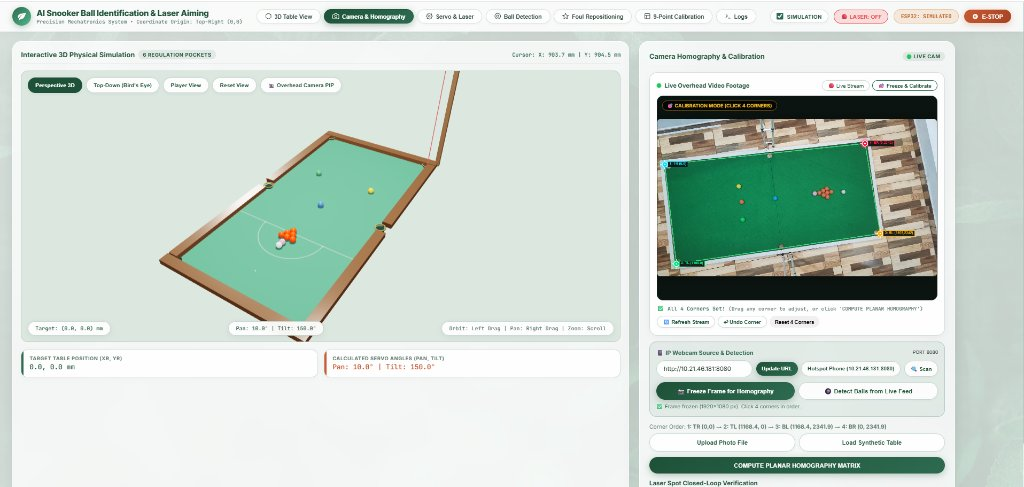
\includegraphics[width=\textwidth]{ui_camera_homography.png}
        \caption{Tab 2: Planar Homography 4-Point Corner Calibration}
        \label{fig:ui_homography}
    \end{subfigure}
    \hfill
    \begin{subfigure}[b]{0.48\textwidth}
        \centering
        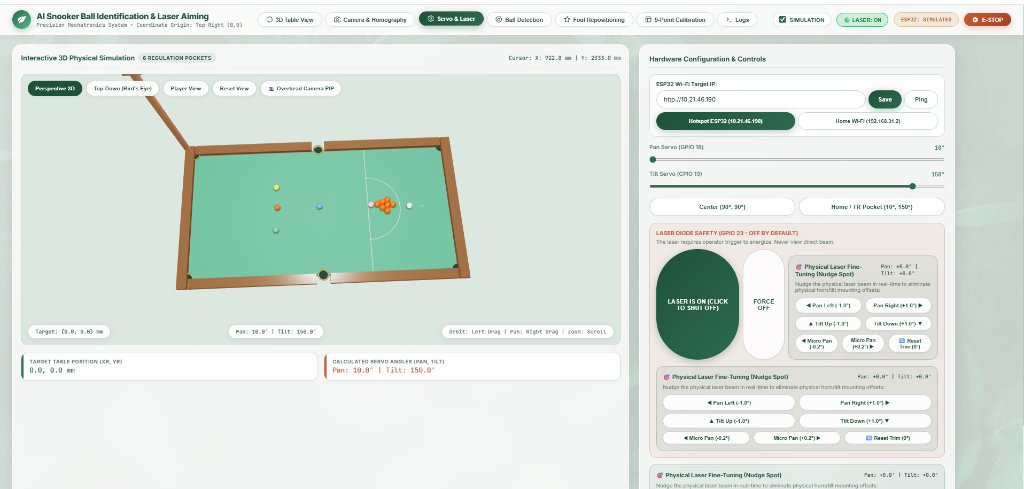
\includegraphics[width=\textwidth]{ui_servo_laser.png}
        \caption{Tab 3: Hardware Servo Sliders and Laser Controls}
        \label{fig:ui_servo}
    \end{subfigure}
    \caption{Web Application Interface: Calibration and Hardware Controls}
    \label{fig:ui_views_2}
\end{figure}

\begin{figure}[H]
    \centering
    \begin{subfigure}[b]{0.48\textwidth}
        \centering
        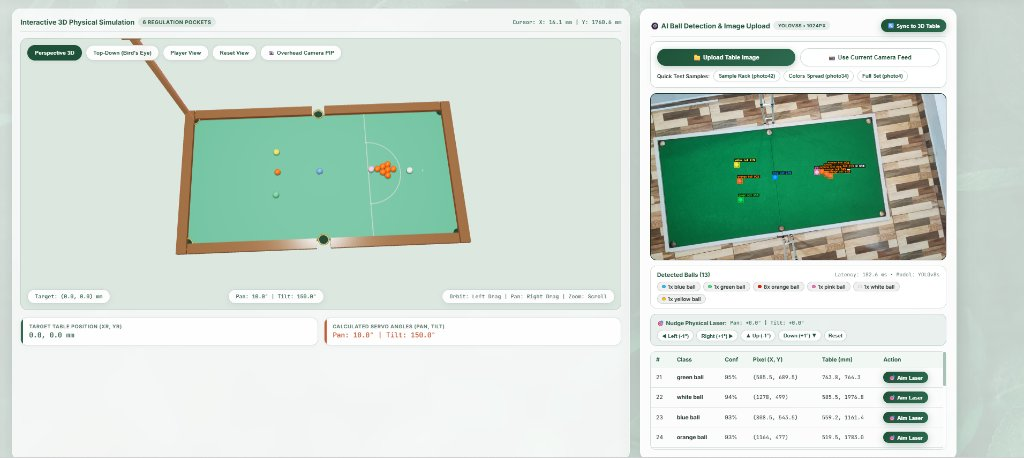
\includegraphics[width=\textwidth]{ui_yolo_detection.png}
        \caption{Tab 4: YOLOv8s Multi-Ball Detection and Metric Localization}
        \label{fig:ui_yolo}
    \end{subfigure}
    \hfill
    \begin{subfigure}[b]{0.48\textwidth}
        \centering
        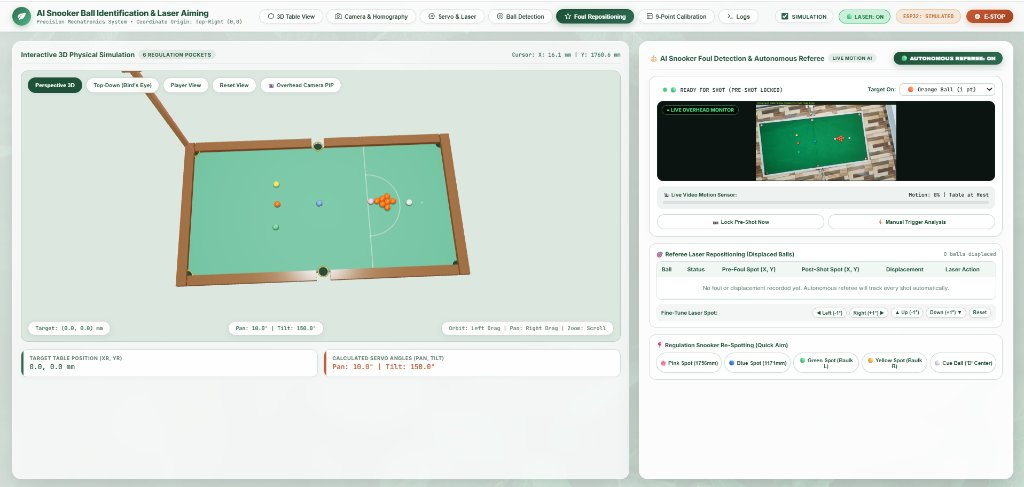
\includegraphics[width=\textwidth]{ui_foul_referee.png}
        \caption{Tab 5: Autonomous Referee and Displaced Ball Table}
        \label{fig:ui_referee}
    \end{subfigure}
    \caption{Web Application Interface: Deep Learning Detection and Autonomous Referee}
    \label{fig:ui_views_3}
\end{figure}

\begin{figure}[H]
    \centering
    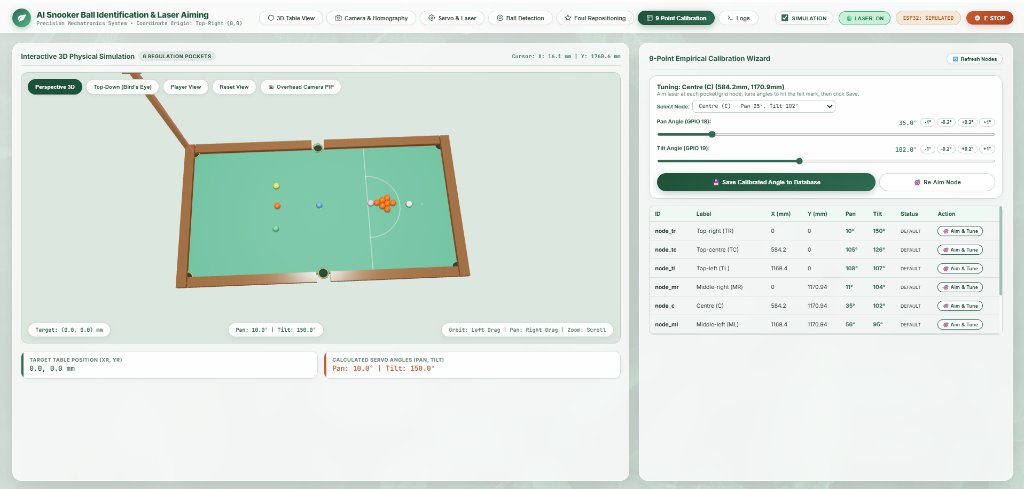
\includegraphics[width=0.65\textwidth]{ui_9point_calibration.png}
    \caption{Tab 6: 9-Point Empirical Calibration Wizard for 2D Bivariate Spline Mapping}
    \label{fig:ui_calib}
\end{figure}

\section{Automated Foul Detection and Referee Engine Implementation}
The autonomous referee engine operates seamlessly in the background without requiring continuous manual interaction:
\begin{enumerate}
    \item \textbf{Optical Motion Analysis:} The engine continuously calculates the absolute difference between successive grayscale frames:
    \begin{equation}
        \Delta I_t = \frac{1}{W \times H} \sum_{x, y} |I_t(x, y) - I_{t-1}(x, y)|
    \end{equation}
    When $\Delta I_t < 0.5\%$, the table is considered static, and the current ball coordinates are automatically cached as the \textit{Pre-Shot Baseline}.
    \item \textbf{Shot Triggering and Settlement:} When a player strikes the cue ball, $\Delta I_t$ surges ($>5.0\%$), transitioning the referee engine into the \textit{Shot In-Progress} state. Once all balls cease moving and $\Delta I_t$ falls back below $0.8\%$ for $2.5\,\text{consecutive seconds}$, the \textit{Settlement} trigger fires.
    \item \textbf{Post-Shot Capture and State Differencing:} A high-resolution post-shot frame is acquired, YOLOv8s extracts all ball locations, and the Hungarian matching algorithm compares post-shot balls against the pre-shot cache.
    \item \textbf{Restoration Workflow:} If the referee calls a foul, the UI highlights displaced balls in red and populates the restoration table with exact pre-foul coordinates $(X_i^{\text{pre}}, Y_i^{\text{pre}})$. Clicking ``Aim Laser'' drives the physical pan-tilt gimbal to project the laser dot onto the cloth, allowing the referee to place the ball directly onto the illuminated spot with millimeter precision.
\end{enumerate}

\section{System Testing}
To verify subsystem correctness and end-to-end reliability prior to live match trials, systematic unit and integration testing were conducted across all hardware and software components.

\subsection{Unit Testing}
\begin{itemize}
    \item \textbf{Homography \& Parallax Math Tests:} Synthetic 4-point corner correspondences and elevated sphere centroids ($Z_{\text{ball}} = 26.25\,\text{mm}$) were evaluated against analytical ground truth in Python/NumPy, confirming sub-millimeter inverse projection error ($<0.05\,\text{mm}$ numerical residual).
    \item \textbf{2D Bivariate Spline Tests:} `scipy.interpolate.RectBivariateSpline` interpolation across the 9-point grid was verified for boundary clamping (`pan` $\in [0^\circ, 180^\circ]$, `tilt` $\in [0^\circ, 180^\circ]$) and smooth continuity across all table quadrants.
    \item \textbf{Hungarian Bipartite Assignment Tests:} Pre/post-shot synthetic coordinates involving identical orange ball swaps, cluster scatters, and pocketed balls were tested to confirm $100\%$ correct stationary, displaced, and potted classification.
    \item \textbf{ESP32 Firmware Endpoint Tests:} Direct HTTP `POST /move` and `GET /laser` calls to `10.21.46.190` validated $50\,\text{Hz}$ PWM servo articulation, IRFZ44N MOSFET switching without brownout resets, and the $120\,\text{s}$ safety watchdog auto-shutoff.
\end{itemize}

\subsection{Integration Testing}
End-to-end integration tests validated live camera stream ingestion, offline fallback caching (`photo58.jpg`), YOLOv8s inference, homography rectification, spline angle dispatch, and Three.js 3D twin synchronization. Table \ref{tab:unit_integration_tests} summarizes the executed test suite.

\begin{table}[H]
\centering
\caption{Automated Unit and Integration Test Execution Summary}
\label{tab:unit_integration_tests}
\resizebox{\textwidth}{!}{
\begin{tabular}{|c|l|l|c|}
\hline
\textbf{Test ID} & \textbf{Module / Pipeline Stage} & \textbf{Verification Criteria} & \textbf{Status} \\
\hline
UT-01 & Homography SVD Solver & 4-point DLT matrix inversion residual $<0.05\,\text{mm}$ & PASS \\
UT-02 & Elevation Parallax Module & Radial shift reduction at table corners ($\gamma = 0.98004$) & PASS \\
UT-03 & 2D Bivariate Spline & Smooth angle interpolation across 9-point grid knots & PASS \\
UT-04 & Hungarian Bipartite Matcher & Accurate Stationary / Displaced / Potted classification & PASS \\
UT-05 & ESP32 REST \& Servo PWM & Response $<50\,\text{ms}$ on \texttt{10.21.46.190} without reset & PASS \\
IT-01 & Offline Frame Resilience & Graceful fallback to cached frame when camera disconnects & PASS \\
IT-02 & Autonomous Referee FSM & Pre-shot lock $\rightarrow$ motion $\rightarrow$ 2.5s settle $\rightarrow$ diffing & PASS \\
IT-03 & End-to-End Laser Restoration & Camera detection to physical laser spot within $\pm 3.0\,\text{mm}$ & PASS \\
\hline
\end{tabular}
}
\end{table}
